\documentclass{jsarticle}
\usepackage[dvipdfmx,hiresbb]{graphicx}

\begin{document}

\title{音楽再生と時間の関係}
\author{藤賀雄太}
\date{2012年12月1日}
\maketitle

\section{イントロダクション}
\subsection{世の中の現状分析}
音楽記録メディアはデジタル化によって小型化が進み、携帯可能な小さな機器(以後、モバイルプレイヤーと呼ぶ)になった。
ウォークマンやiPodを代表とする再生専用機器は広く普及したが、最近では、携帯電話と一体型になっているものも広く普及しており、音楽再生機器をどこでも持ち歩けるようになった。
また、スピーカーではなく、ヘッドホンで聴く場合、自分だけ聴くことができるため、例えば電車の中などの公共空間で聴くことや、学校の授業の合間の時間にすぐに取り出して聴けるようになった。そのため、音楽を聴く場所と時間に制約がなくなり、いつでもどこでもなんでも聴くことができるようになった。


\subsection{そこから見えてくるチャンスと問題点いくつか}
一方、生活のコンテキスト(時間や場所の情報)から音楽をリコメンドするものはあまりみつけられなかったが、楽曲の音楽の情報自体にアクセスするのではなく、楽曲が再生される状況の関係性から楽曲を分析することができるのではないかと考えた。
\subsection{研究課題}
人によって、生活が不規則な人もいると容易に推測できるために、時間によって、傾向が出ないことも考えられる。必ずしも。時間と音楽の再生に相関がある人ばかりではないことも留意しつつ、調べる必要がある。そのため、音楽の再生時刻だけでなく、普段の生活がどのようになっているのかを直接知る必要がある。また、ランダム再生(=シャッフル再生)機能が広く普及しており、再生履歴も一元的にユーザーによる積極的な選択としてみなすことが出来ない場合も注意する必要がある。また、ソフトの仕様により、履歴情報が全て記録されていない場合があり、今回使用したAppleによるiTunesという音楽再生プレイヤーは、ひとつの楽曲に対して、最後に再生した時刻だけしか記録されていない。全てを保存するアプリケーションを自作することも可能だったが、その場合、従来の音楽再生の体験自体を大きく変化させてしまうことによって、従来の履歴情報を取得することが困難になると考えたため、この点においては妥協してiTuensを使用することにした。
また、今回はAppleのiTuensという音楽再生プレイヤーに限定して分析した。そのため、実際に音楽を再生するまでにかかる工程が、iTuensのユーザーインターフェースに依存してしまうため、他の音楽再生プレイヤーで得られた履歴情報とは偏りが出来る可能性がある。
\subsection{先行研究}
産総研の後藤真孝さんのMusicreamのように、インターフェースによって音楽を選択する支援をするものや、楽曲のジャンルの関連性を取得するgeniusなどのサービス、また、ユーザーが楽曲から受ける印象を集めることで、音楽の印象から、気分にあった音楽を選ぶことのできるmusicoveryなどのサービスがある。

\subsection{研究動機}

以前は例えば自宅で夜、音楽鑑賞するといった決まった状況で聴いていたため、音楽を再生する状況に外的な別段の変化はなかった。
しかし、モバイルプレイヤーにおける音楽の再生は、場所や時間を選ばない。そのため、モバイルプレイヤーの使用者は様々な場所や時間において、自分で音楽を再生する音楽を選択する必要がでてきた。
ユーザーは、状況が変化すると、音楽を再生する同期や気分などに差が大きく出ると思われる。
そこで、私は、外的な状況の変化に対して、音楽の再生がどのように変化しているのかを調べることにした。
\subsection{方針}
本研究では特に時刻に注目して、時刻によって音楽の聴き方がどのように変化するのかを調べた。
時刻に注目した理由は以下の通りである。
\begin{itemize}
\item
規則的、周期的である。ほとんどの場合、朝は自宅から始まり、夜は再び、自宅にもどる。その時間も人によってではあるが、パターン化されていると考えられる。そのため、時刻だけからもある程度、人の営みを推測することができそうだと推測できた。
\item
音楽と相関がありそうである。現状で、朝の音楽や、オールナイトコンサート、夜のジャズクラブなど、時間を冠した音楽のシーンは見慣れている。そのため音楽には時間的な要素が存在していると予測できた。
\end{itemize}

\subsection{期待される成果}
この研究が音楽の自動選曲システムの向上に貢献できればと考える。研究の結果、時間情報はfoobarでした。
\subsection{キーワード}
iTunes, iPod, 時間情報, レコメンドサービス, ライフログ

\section{分析手順}
\begin{enumerate}
\item
被験者10名(iTunesをいつも利用して音楽を聴いている大学生)から履歴ファイル(xmlファイル)をメール添付でもらう。

\item
被験者に自分の生活を曜日毎にアンケートシートに書いてもらう。
\begin{center}
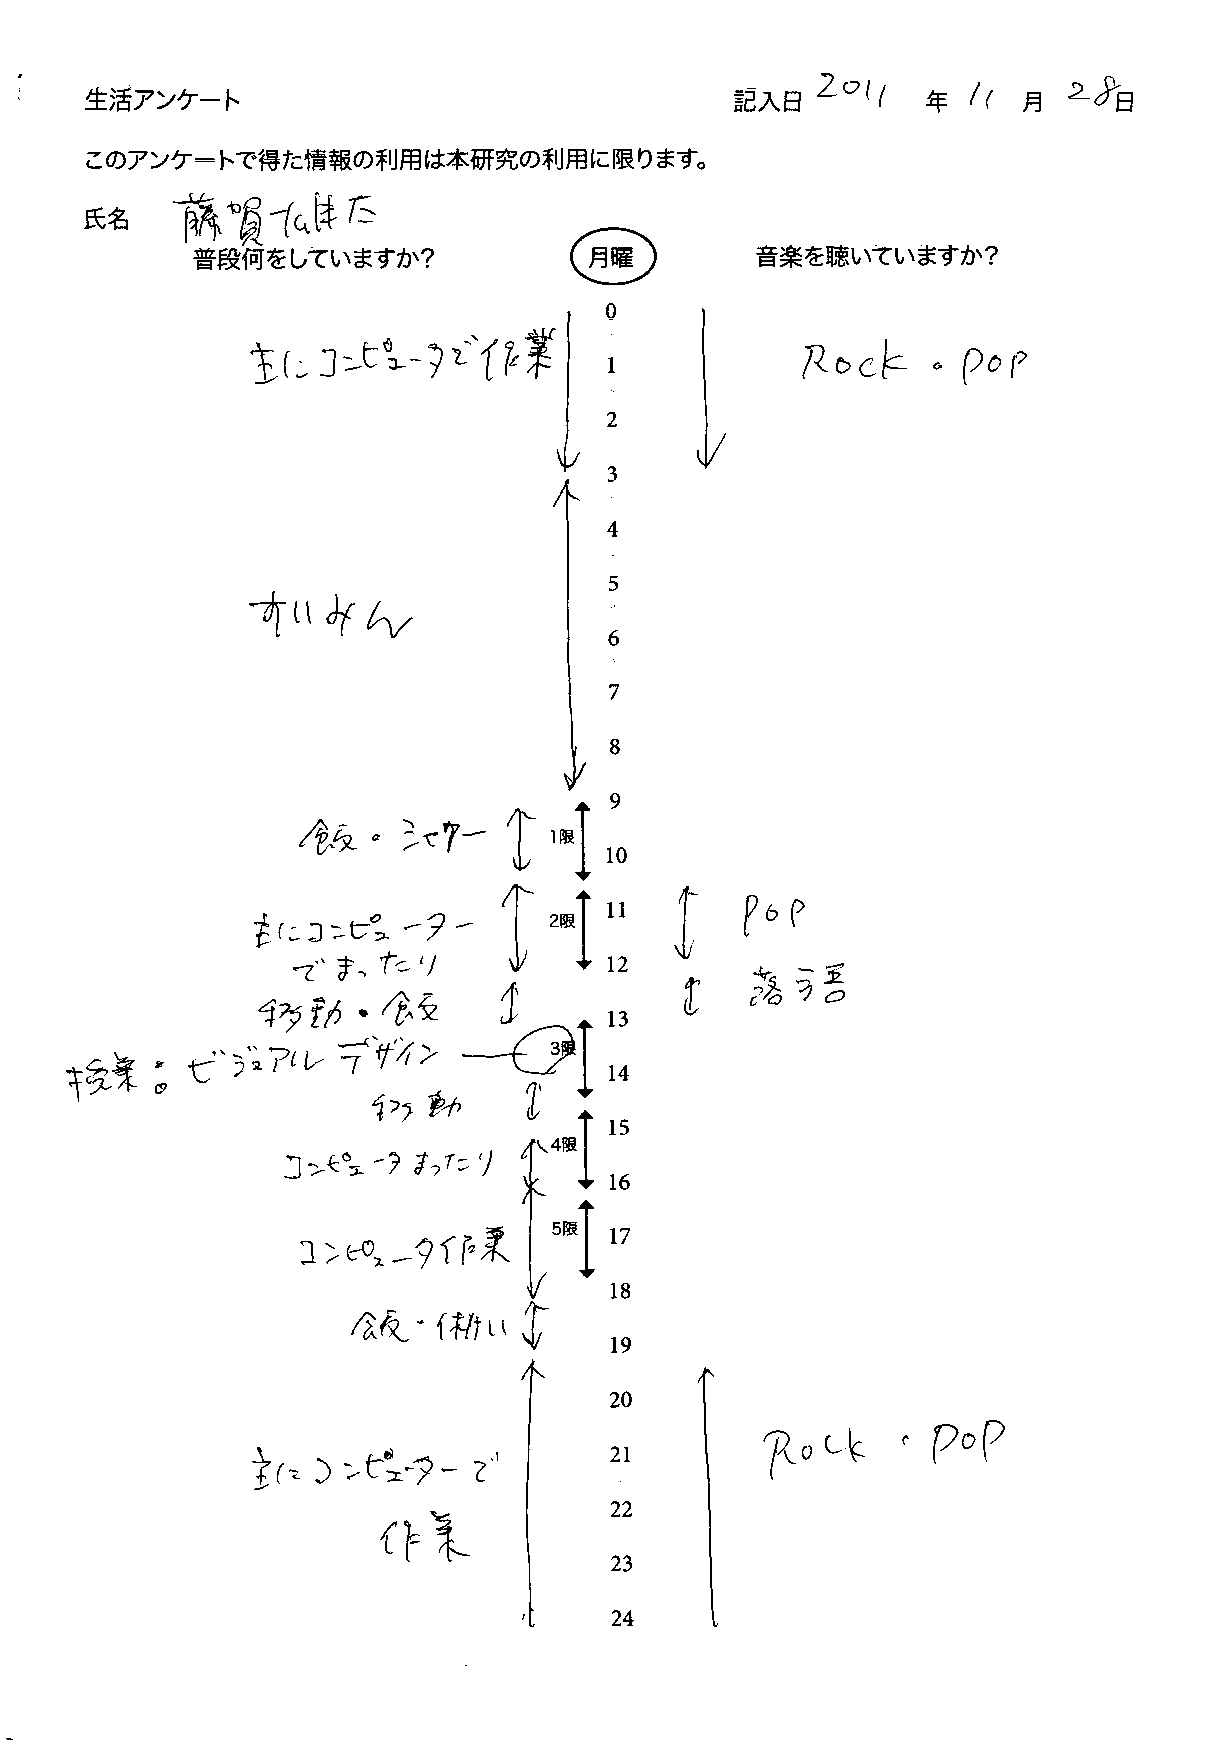
\includegraphics[width=7cm]{musicLifeSheet_sample.pdf}
\end{center}

被験者に渡したのは、0時から24時までを30分刻みで目盛りを付けたもので、普段の生活と、普段の音楽聴取を記入してもらうもので、月曜日から日曜日までの合計7枚のものである。
不規則な生活、気まぐれな音楽再生など、毎週規則正しく定期的に書けない部分も備考として記入してもらう。
なお、iTunesをシャッフルで聴いたかどうかは、iTunesに記録されていないため、備考に書いてもらう。
\item
pythonを用いて、履歴ファイルから、以下の情報だけを読み取って、テキストファイルに書き出す。
\begin{itemize}
\item
楽曲のジャンル
\item
最後に聴いた日付・時間
\item
再生回数
\end{itemize}

\item
Rを用いて、2でつくったテキストファイルを読み込んで、一度以上再生された楽曲について、曜日毎に分類し、さらに、0時から24時まで1時間刻みのヒストグラムをつくる。そして、ヒストグラムのデータをcsvファイルとして保存する。なお、ヒストグラムを画像ファイル(pngデータ)として書き出す。

\item
openFrameworksを用いて、csvファイルから、0時から24時まで30分刻みのヒストグラムを月曜から日曜までの累積棒グラフの形式でつくる。棒グラフの棒の数は、24(1時間刻み)*7(月曜から日曜)=168本になる。総合再生回数がベスト5のものだけをカラーにして、それ以外をその他としてグレーで描画した。

\begin{center}
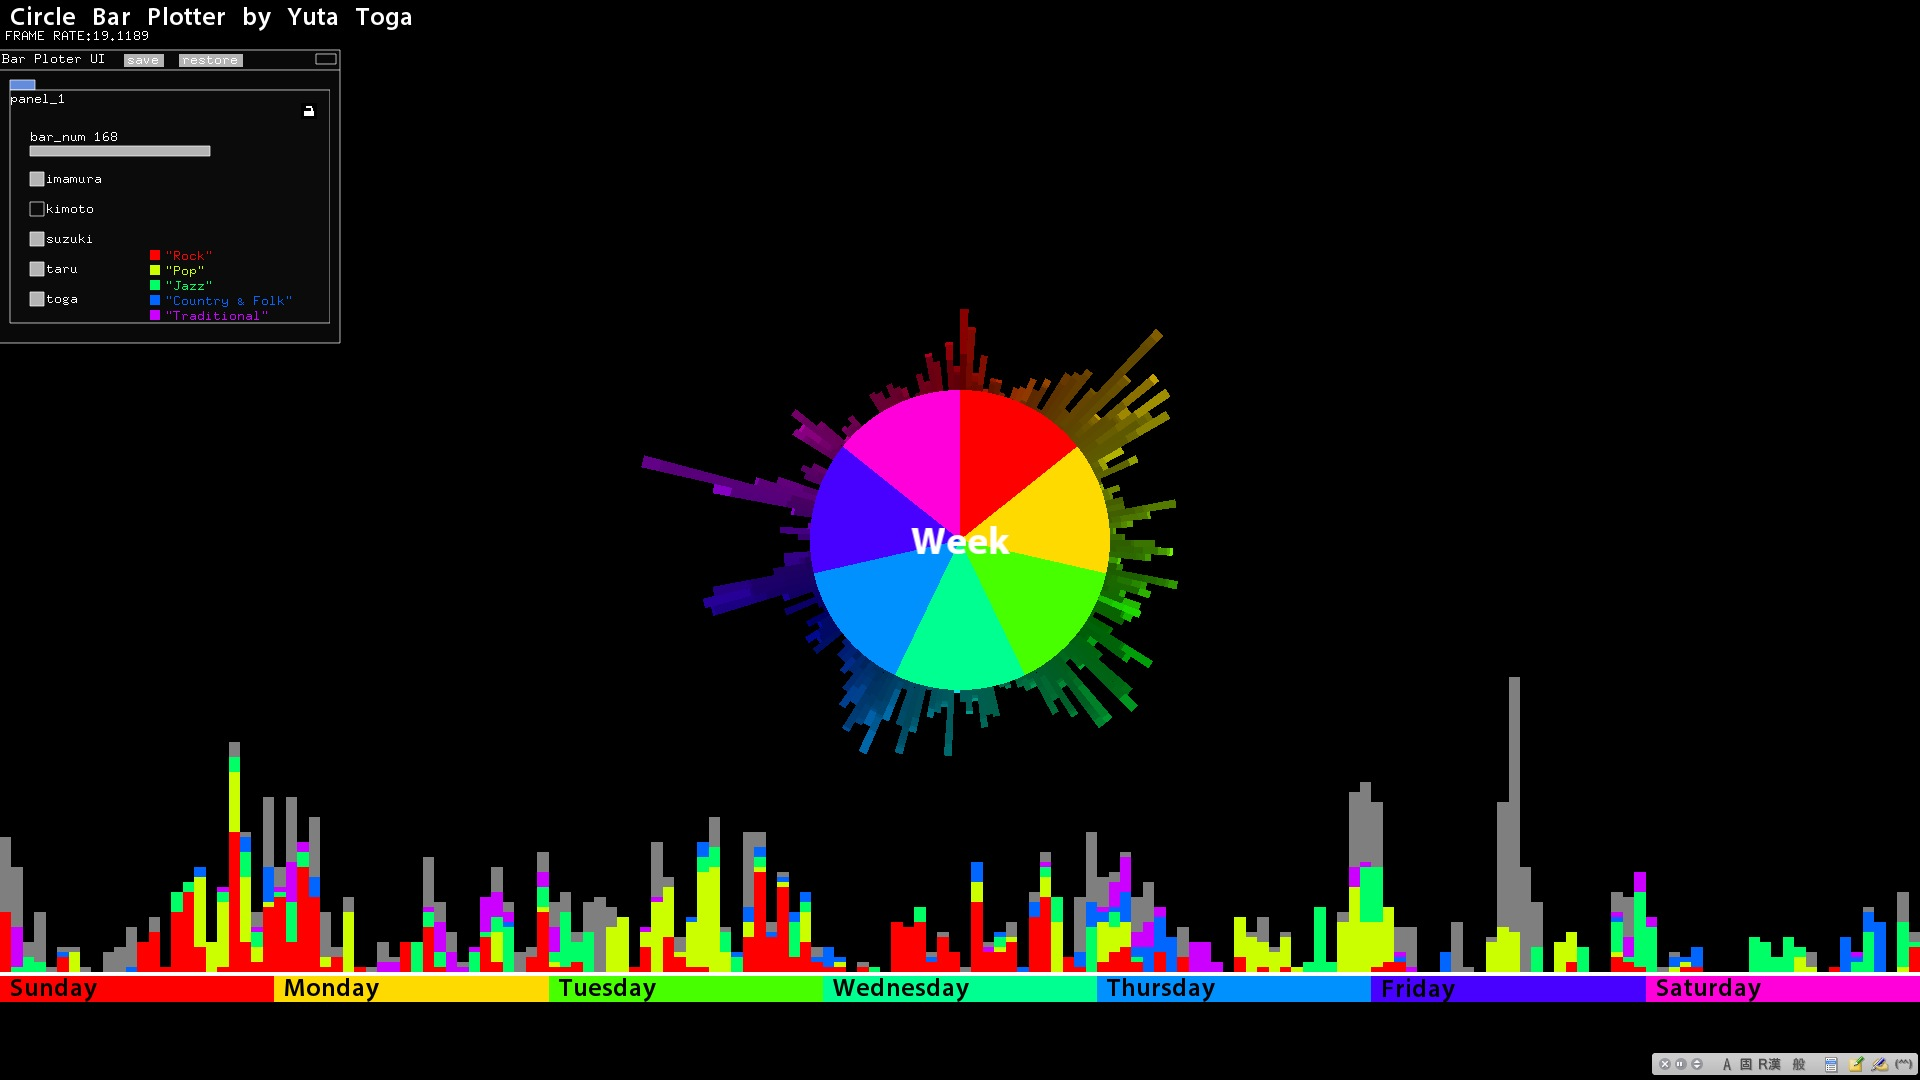
\includegraphics[width=14cm]{graph_sample.jpg}
\end{center}

\item
ヒストグラムの見た目から、聴いている音楽と、時間に相関があるかを調べる。

\item
被験者のアンケートシートで得た情報と、xmlファイルから読み取ったものとの比較を行う。

\item
質問があったらインタビューを行う。

\end{enumerate}

\section{結果}
ヒストグラムはこうなりました。寝ている時間が推測できる。必ず聴いていない時間が存在することがあり、その時間は定期的な会議などがあることが多かった。金曜の夜だけ多く聴いているというような、曜日による偏りが見られた。

\section{分析}
iTunesの仕様により、再生履歴は最後に聞いた時間の情報しか残っていない。すなわち、10回聞いたの楽曲がある場合も、いつ聞いたのかという情報は最後の10回目しか記録されておらず、1回目から9回目の情報は上書きによって失われている。そのため、今回の研究では、アンケートにおいて、シャッフルで再生しているかどうかを聞き出すことにした。
 もし、月曜日に特に音楽を聞いているという場合、なぜ月曜にそうなるのかという理由は聴いてみないとわからないため、アンケートで得られた、普段の生活を参照した。
また、この時間あなたは授業などで音楽を聴けない状況ではないですか?というようにインタビューによって利用者の音楽試聴状況を推測することができた。これは、今後、自動選曲システムにおいて、設定をすべてユーザーに任せるのではなく、もしかして、金曜の夜はあまりロックは聴かないですね?というような、質問形式で数問回答させることにより、ユーザーの音楽試聴状況に沿った選曲ができる(沿うことがよいリコメンドかどうかは別として)可能性を示唆する。
ランダムに再生している人と、時間と音楽再生に偏り(相関がある)人にどう分かれるのかを調べる。

\section{考察}
アンケートに書かれていることと、xmlファイルから得られた音楽再生の状況が異なる場合、一致する場合それぞれについて、なぜそうなるのかを考察する。
生活のコンテキスト、特に時間情報が音楽再生に影響力をもっているかどうかを考察し、音楽リコメンドサービスについての発展を考える。

\section{備考}
研究資料および、プログラムの一部は、(個人情報は含まない)
yutatoga.com/thesisからダウンロードできる。


\end{document}